\documentclass[letterpaper, 12pt]{article}
\usepackage[margin=1in]{geometry}
\usepackage{amsmath}
\usepackage{amssymb}
\usepackage{xcolor}
\usepackage{graphicx}
\usepackage[center]{caption}
\usepackage{hyperref}
\usepackage{fancyhdr}

\pagestyle{fancy}
\fancyhf{}
\rhead{
    Shendong Li
    Table 7
    Calc 1
}
\rfoot{
    Page \thepage
}

\usepackage{indentfirst}
\setlength{\parindent}{2em}

\begin{document}
\title{Avocado: Of Duty or Ambition?}
\author{by Shengdong Li}
\date{14 April 2020}
\maketitle
\section{Backstory (you can skip this if you want)}
$2168.9$, the world is a dark, foreboding place. The streets are littered with tomatoes, cucumbers, and eggplants, all burning, spoiling and releasing a smell akin to rancid oil. Buildings lay sideways, half demolished, their broken materials sprinkled all over the ground like cheese on a good pizza. Above, the day is perpetually overcast with gray smog, a dark blanket of negligence, leaving the problems of the city to fester. \par
Bob crouches behind the one solitary wall left standing of a small house, brusquely sharpening a kitchen knife atop a smooth block of a whetstone. He is cold, tired, and hungry, a typical set of feelings for a citizen of Fruit city. Occasionally he sets the knife down and rubs his eyes, holding back tears and coughing from the burnt organic smell drifting about the city \par
It has been $68.9$ years since the evil bananas, spawned from an intense amount of radiation, took over human civilization, and began to persecute all other fruits and vegetables. While the bananas weren’t initially hostile towards humans, the loss of fruit and veggies as a food source forced humanity to fight a war of attrition with them in order to survive. A war that the humans are losing terribly. \par
Because of the current status quo, you might think that Bob has lost all hope, and has become a madman sharpening his knife, physiological state bent out of shape. And you might’ve been right—had Bob not found the last fruit alive in Fruit city, $.9$ years ago. \par
You see, Bob, the legend himself, has a plan. The half-life of a radioactive banana is $70$ years. Fruit city is the headquarters of the evil banana republic, and once the period of $70$ years ends, the bananas will be significantly weakened. Bob has already infiltrated the area around headquarters successfully. If he manages to stay alive for $1.1$ more years, he might be able to slice and dice his way into the fruit headquarters and slay the evil Bananaking, along with all his evil ambitions and desires. \par
The avocado that he found gave him tremendous sustenance, such that he has already lasted $.9$ years with only half of the avocado. If he has lasted $.9$ years previously, he might be able to live on for $1.1$ more years. However, the avocado has been speaking to him ever since that fateful day: “Run away from Fruit city, and start a new life with me! Revenge means nothing if it means humankind runs out of a source of food anyway. With half a slice, I can still grow!” \par
But Bob had already come this far. Going back would mean putting down his pride, risking encounters with more bananas, and turning back on all the meaning that his life had had thus far. It would be crazy to run away now. But maybe he \textit{was} crazy: who had ever heard of a talking avocado? \par
\section{Problem}
Over the past $.9$ years, Bob had been calculating his chances, in a perpetual state of anxiety. Based on his data, Bob discovered that he \textbf{consumes} about $13\:cm^3$ of avocado every $.1$ years. His scans of the avocado by his \textit{secret scam scanner} revealed that the base of the half a slice of avocado was bound by an \textbf{ellipse} of equation $\frac{\left(x-1\right)^{2}}{6^{2}}+\frac{y^{2}}{3.5^{2}}=1$. The pit of the avocado was also an \textbf{ellipse} of equation $\frac{\left(x-.5\right)^{2}}{2.85^{2}}+\frac{y^{2}}{2.3^{2}}=1$. However, Bob's scanner broke before it could consider the $z-$axis (what a scam), and integrate the value of the cross-sections of \textbf{semicircles} perpendicular to the $x-$axis.\par
\begin{figure}[h]
    \begin{center}
        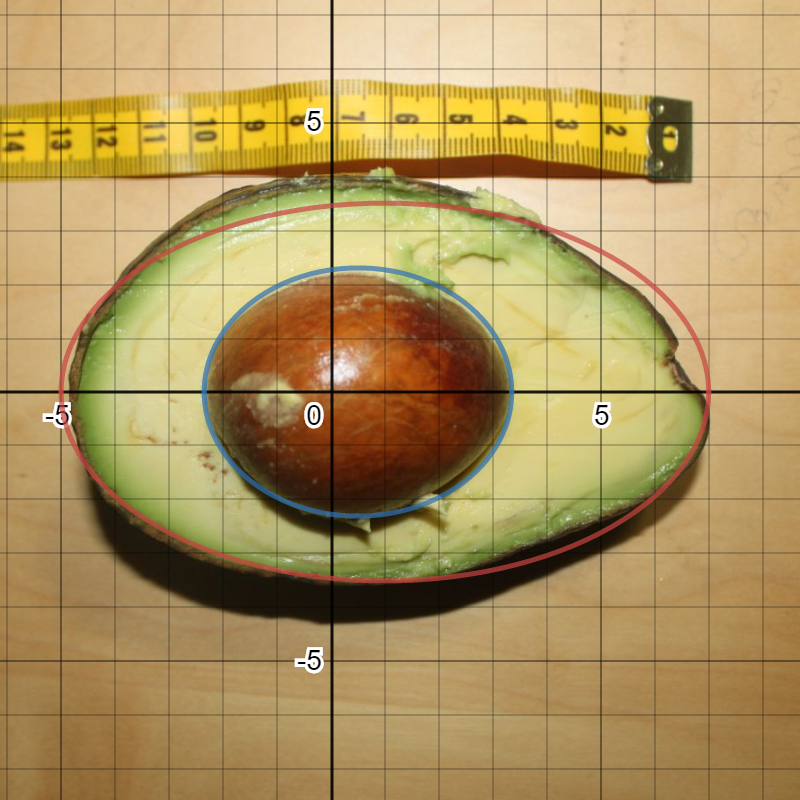
\includegraphics[scale=.3]{avocad.png}
        \caption{\textit{Picture of the fated avocado.} Desmos link \href{https://www.desmos.com/calculator/i0kemx2ihg}{\textcolor{blue}{here}}, or see embed below}
    \end{center}
\end{figure}
Whatever the case, all this uncertainty would be put to rest, because Bob had made a resolution: should he be guaranteed to live \textbf{1.1} years with the amount of avocado that he has left, he will choose to stay in Fruit city. However, if it is certain that he cannot survive for that long, then maybe he should finally listen to the avocado for once. \textbf{Should Bob stay in Fruit city, fulfilling his quest for revenge once and for all, or leave it, turning back on everything that he holds dear?}
\end{document}